% 	This template is  MIT licensed.

% 	Basic file to demonstrate the usage of this LaTeX template.
% 	You can build your own paper/thesis on top of this file.
% 	Simply adjust the document class and all metadata and start working.
%
\documentclass[
	language=english, % set to english or german
	type=bachelor, % set to bachelor, master or seminar
]{isthesis}

% Graphics rendering using TikZ
% See: https://en.wikibooks.org/wiki/LaTeX/PGF/TikZ
\usepackage{tikz}
% Include required TikZ libraries here, some exemplary libraries are pre-included
\usetikzlibrary{calc}
\usetikzlibrary{matrix}
\usetikzlibrary{positioning}
\usetikzlibrary{shapes.geometric}

%Add your library here
\addbibresource{library.bib}

% Import acronyms
% \newacronym[longplural={<long plural>}, shortplural={<short plural>}]{<label>}{<short>}{<long>}
% 	label = is the unique identifier and sort key for the acronym, can be the same as <short>
%	short = is the abbreviation or acronym
%	short plural (optional) = is the plural of the abbreviation or acronym
%	long = is the long form of the acronym, this will appear in the list of abbreviations
%	long plural (optional) = is the long plural form of the abbreviation or acronym

\newacronym[shortplural={KMUen}, longplural={Kleine und Mittlere Unternehmen}]{kmu}{KMU}{Kleines und Mittleres Unternehmen}
\newacronym{CD}{CD}{Corporate Design}
\newacronym{SQL}{SQL}{Structured Query Language}
\newacronym{FAU}{FAU}{Friedrich-Alexander-Universit\"at Erlangen-N\"urnberg}
\newacronym{BPM}{BPM}{Business Process Management}
\newacronym{npm}{NPM}{Node Package Manager}
\newacronym{diss}{DISS}{Digital Industrial Service System}

% Import symbols
% Syntax: <Symbol> <Label> <Name>
% The symbols are sorted by their labels
\addsymboltolist{$\Pi$}{Pi}{Projection}
\addsymboltolist{$\Join$}{Join}{Natural Join}
\addsymboltolist{$\sigma$}{Selection}{Selection}


% Import custom commands
% If you want to define custom commands, please do so here
\DeclareUnicodeCharacter{03B1}{$\alpha $}
\DeclareUnicodeCharacter{03B2}{$\beta$}
\DeclareUnicodeCharacter{03B3}{$\gamma$}
\DeclareUnicodeCharacter{03B4}{$\delta$}
\DeclareUnicodeCharacter{03B6}{$\zeta $}
\DeclareUnicodeCharacter{03B7}{$\eta $}
\DeclareUnicodeCharacter{03B8}{$\theta $}
\DeclareUnicodeCharacter{03BA}{$\kappa $}
\DeclareUnicodeCharacter{03BB}{$\lambda $}
\DeclareUnicodeCharacter{03BC}{$\mu $}
\DeclareUnicodeCharacter{03BE}{$\xi $}
\DeclareUnicodeCharacter{03C0}{$\pi $}
\DeclareUnicodeCharacter{03C6}{$\phi $}
\DeclareUnicodeCharacter{03C9}{$\omega $}



% Document meta information
\isthesis{
    title={Development of a web-oriented code modeling the propagation of ultrashort pulses in optical fibre},
    author-name={Hernan Alberto Aguilera Abril}, % Separate multiple authors with commas
    author-email={hernan.aguilera@fau.de},
    %author-phone={+49 1776300853}, % Use international numbers format
    author-matriculation={Matrikelnummer: 22710623},
    % author-address={Erwin Rommel Str. 53},
    % author-zip={91058},
    author-city={Erlangen},
    principal-supervisor={Prof. Dr.-Ing. Bernhard Schmauss}, % This must be a professor
    associate-supervisor={Prof. Dr. Nicolas Joly}, % This is your main supervisor, i.e., a post doc or doctoral student
    tutor-supervisor={}, % If required, define an additional supervisor resp. tutor here
    group={Lehrstuhl für Hochfrequenztechnik},
    group-institute={Friedrich-Alexander University of Erlangen-Nuremberg},
    %studies={B.Sc. Elektrotechnik – Elektronik – Informationstechnik}, %your field of studies, i.e. Wirtschaftsinformatik or International Information Systems
    %
    %associate-group={}, % When the thesis is done in cooperation with another chair, add it here
    %associate-group-institute={}, % add cooperating institute or university here
    seminar={Photonik}, % The title of your seminar
    submission-date={2021-05-01} % The date you handed in your document: Format yyyy-mm-dd
    %primary-logo={}, % Uses the FAU logo by default
    %primary-logo-height={}, % Uses 16mm as default height
    %secondary-logo={}, % Logo of the secondary institution (cooperating chair/university), USES Faculty logo by default
    %secondary-logo-height={} % Uses 16mm as default height
}


\begin{document}
    % Title page
    \newcounter{savepage}
    \maketitle

	% Quote
    % You can put an optional quote page in front of your content
    %   \quotepage[author={Arthur C. Clarke}]{
    %   	        Any sufficiently advanced technology is indistinguishable from magic.
    %   }
    
    % Table of contents
    \tableofcontents

    % List of figures (if you have figures)
    \listoffigures

    % List of tables (if you have tables)
    \listoftables
    
    % List of listings (if you have listings)
	\lstlistoflistings

    % List of abbreviations (if you use acronyms)
    \listofabbreviations

    % List of symbols (if you use symbols)
    \listofsymbols
	
	% Abstract
	%
	% Comment out this part, if you don't require an abstract
	\begin{abstract}
	    % Add your abstract here:
		\lipsum[1]
	\end{abstract}
	
	% storing the last pagenumber
    \setcounter{savepage}{\value{page}}
    
    
    % Content
    \begin{content}
        % Add your content files:
		\chapter{Introduction}
Objective:
Develop a tool for the future students who will study nonlinear optics in fibres so that they can appreciate more easily the different physical processes happening to a short pulse propagating in a dispersive nonlinear medium. These include the influence of the dispersion (second and third order), the self-phase modulation, the emission of dispersive wave, the soliton dynamics. Eventually, the code will be released as a web-interface for the future students to directly modify the physical parameters of the pulse, but also of the fibre.**



This \LaTeX \- template has been developed by the University of M\"unster and adapted by the Chair of Digital Industrial Service Systems at the \gls{FAU} to match the \gls{FAU} \gls{CD}. The file \path{main.tex} is the master file.

It was originally built by  Jan Betzing and Dominik Lekse and draws from the DBIS template by Till Haselmann and Florian Stahl, as well as from the IS template by Stephan Dlugosz. The adaption to FAU was done by Matthias Stierle. Currently, Sebastian Dunzer maintains the template.

This document is work-in-progress and provides instructions on how to use the template. It does not give advices on scientific writing.

Please feel free to contribute to this template.

\paragraph{TODO}
\begin{itemize}
	\item Configuration switch for having \textbackslash chapter\{\} begin on a new page
	\item Replace \texttt{kvoptions} with \texttt{pgfkeys}
\end{itemize}
		\chapter{Modeling of the Group Velocity Dispersion}

First will be the fiber treated as a linear optical medium while considering the pulse-propagation problem, thus it is possible to inspect the effect of GVD under certain circumstances where it dominates over the nonlinearities \citep{ AgrawalBook}. A further objective of this chapter is to implement a code capable of illustrate the Dispersion-induced broadening of optical pulses for Gaussian and "sech" shapes.
		\chapter{Template Features}
This chapter gives examples on what you can do with this template. It's just a brief overview. Please consult the common sources on how to write scientific documents and documents with \LaTeX.

\section{Structure}
This template provides three structural levels that appear in the table of contents: \texttt{\textbackslash chapter}, \texttt{\textbackslash section}, and \texttt{\textbackslash subsection}. Chapters will always start on a new page. Additionally, you can use \texttt{\textbackslash subsubsection} and \texttt{\textbackslash paragraph} as non-hierarchical means to structure your thesis.


\subsection{Lists}
You can use the default \LaTeX \- functions for writing lists, viz., \texttt{\textbackslash enumerate} for numbered lists and \texttt{\textbackslash itemize} for bullet point lists. Again, the \texttt{\textbackslash subsubsection} and \texttt{\textbackslash paragraph} can be used as structural elements, e.g., when listing definitions of terms.

\subsection{Footnotes}
Footnotes are continuously numbered throughout the document. Use the \texttt{\textbackslash footnote\{text\}} command.  They appear on the page their reference is on \footnote{This is an exemplary footnote.}. Footnotes have to be placed without whitespace behind the word and within the sentence boundaries, i.e., before the period.

\subsection{ToDo-Notes}
You can use ToDo notes using the \texttt{\textbackslash todo\{text\}}  command. Please make sure to remove any ToDo notes before handing in your thesis! \todo[inline]{ToDo: Remove me before publishing}

\section{Formatting Text}
\LaTeX \- provides \texttt{\textbackslash textit\{text\}} for \textit{italics}, \texttt{\textbackslash textbf\{text\}} for \textbf{bold face}, \texttt{\textbackslash texttt\{text\}} for \texttt{typewriter}, \texttt{\textbackslash textsc\{text\}} for \textsc{small caps}, \texttt{\textbackslash underline\{text\}} for \underline{underline}. Additionally, the template provides  \texttt{\textbackslash texthl\{text\}} for \texthl{highlighted text}. Please remove any highlighted text before handing in your thesis!

Please use the \texttt{\textbackslash enquote\{text\}} command for \enquote{direct quotes}.

\subsection{Colors}
This template comes with the colors defined in the \gls{CD} of the \gls{FAU}. Table \ref{tab:colors} lists the color names. You can apply them to text by using the  \\ \texttt{\textbackslash textcolor\{color name\}\{text\}} command.
	
\begin{table}[caption={Colors defined by the template}, label=tab:colors]
	\centering
		\begin{tabular}{@{}ll@{}}
			\toprule
			{\bf Color Name} & {\bf Result} \\ \midrule
			fau-grey      & \textcolor{fau-grey}{Exemplary Text and 0123456789}  \\
			fau-red      & \textcolor{fau-red}{Exemplary Text and 0123456789}  \\
			fau-blue      & \textcolor{fau-blue}{Exemplary Text and 0123456789}  \\
			fau-cyan    & \textcolor{fau-cyan}{Exemplary Text and 0123456789}  \\
			fau-orange      & \textcolor{fau-orange}{Exemplary Text and 0123456789}  \\
			fau-green      & \textcolor{fau-green}{Exemplary Text and 0123456789}  \\ \midrule
		\end{tabular}
\end{table}


\section{Figures}

The \texttt{figure} environment is wrapped around images. These images should either be included as PDF-file via \texttt{\textbackslash includegraphics}, or created via \textit{TikZ/PGF}. For included images, make sure to use high-resolution images, preferably vector images.

Figures float, i.e., they do not necessarily appear at exact the same position you have defined them. Make sure to set a  \textit{caption} and an optional \textit{label} as figure parameters. 

\begin{figure}[label={fig:img01}, caption={Relationship of students and theses}]
  %  \caption*{Source: Some Source}
	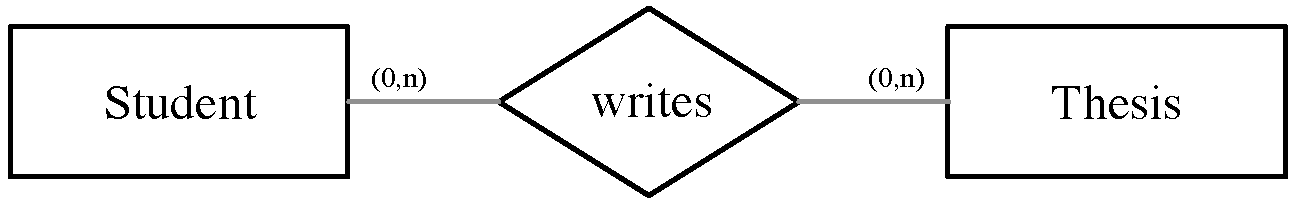
\includegraphics[width=.6\textwidth]{figures/figure01.pdf} 
\end{figure}


\subsection{Subfigures}
Sometimes it might be handy to contrast figures, i.e., by placing them next to each other. The template uses the \textit{subcaption} package to provide subfigures. The following example contains two figures, where each subfigure has its own \texttt{\textbackslash label} and \texttt{\textbackslash caption}. Additionally, the whole figure has its own \textit{caption} and \textit{label}. That means, you can reference subfigures  Figure \ref{fig:subfig1} and Figure  \ref{fig:subfig}. Only the whole figure will be listed in the table of figures.

Subfigures are not limited to images, but may also include listings or tables. Figure \ref{fig:subfig} shows a sample database query expressed in \gls{SQL} (Figure \ref{fig:subfig1}) and as query plan in relational algebra  (Figure \ref{fig:subfig2}).
 
\begin{figure}[caption={Exemplary use of subfigures}, label={fig:subfig}]
	
	\begin{subfigure}[b]{.45\textwidth}
		
		\begin{lstlisting}[nolol, language=SQL]
		SELECT b, d FROM 
			EXAMPLE.RELATION1 r,
			EXAMPLE.RELATION2 s,
		WHERE 
			r.a = 'c'
		AND 
			s.e = 2
		AND 
			r.c = s.c; 
		\end{lstlisting}
		\caption{\gls{SQL} select statement}\label{fig:subfig1}
	\end{subfigure}
	\begin{subfigure}[b]{.53\textwidth}
		\centering	
		\begin{tikzpicture}[node distance = 2cm, auto,
		database/.style={
			cylinder,
			cylinder uses custom fill,
			cylinder body fill=gray!30,
			cylinder end fill=gray!20,
			shape border rotate=90,
			aspect=0.25,
			draw
		}]
		\node [] (queue) {$\Pi_{b, d}$};
		\node [below of=queue] (join) {$\Join_{r.c = s.c}$};
		
		\node [below left of=join,xshift=-1cm] (l1) {$\sigma_{r.a = 'c'}$};
		\node [database, below of=l1] (l2) {\texttt{r}};
		
		\node [below right of=join,xshift=1cm] (r1) {$\sigma_{s.e = 2}$};
		\node [database,below of=r1] (r2) {\texttt{s}};
		
		\draw [<-] (queue) -- (join);
		\draw [<-] (join) -- (r1);
		\draw [<-] (r1) -- (r2);
		\draw [<-] (join) -- (l1);
		\draw [<-] (l1) -- (l2);
		\end{tikzpicture}
		\caption{Sample evaluation plan}\label{fig:subfig2}
	\end{subfigure}
\end{figure}
\section{Listings}
You can use listings to typeset source code. This template uses the \textit{listings} package. Wrap code inside the \texttt{lstlisting} environment and set the \textit{language} (e.g., Java, SQL), \textit{caption}, and optional \textit{label} parameters. If the source code highlighting highlights the wrong keywords or misses keywords, use the \textit{deletekeywords} resp. \textit{morekeywords} parameters. Consult the package documentation for further information.

\begin{lstlisting}[float=htp, caption={Euclid's GCD algorithm implemented in Java}, label={lst:euclid}, language=Java, deletekeywords={}, morekeywords={}]
public class Euclid {

	public static int gcd(int p, int q) {
		if (q == 0) return p;
		else return gcd(q, p % q);
	}

}
\end{lstlisting}

\section{Algorithms}
Some users might require specifying algorithms. This template uses the \textit{algorithm}, \textit{algorithmicx}, and \textit{algopseudocode} packages. Consult the respective manuals for further information. Algorithms do not appear in a table at the beginning of the document, i.e., there is no list of algorithms.

\begin{algorithm}[htb]
	\begin{algorithmic}
		\Require nonnegative integer $a$, nonnegative integer $b$
		\Function{Euclid}{$a, b$}
		\If {$b = 0$} \Comment{comment}
		\State{return $a$;}
		\Else 
		\State {return \textsc{Euclid}$(b, a\mod b)$;}
		\EndIf
		\EndFunction
	\end{algorithmic}
	\caption{Euclid's GCD algorithm in pseudocode}
	\label{alg:garbage}
\end{algorithm}

\section{Acronyms and Abbreviations}
This template provides comprehensive support for acronyms and abbreviations. The template uses the \textit{glossaries} package. 
Please do only define abbreviations and symbols that are uncommon. That means, common abbreviations such as \enquote{e.g.} or \enquote{i.e.} should not be listed. Abbreviations and symbols are sorted automatically by their label. 

\subsection{Custom Abbreviations}
Custom abbreviations are defined in the \path{config/acronyms.tex} file, using the \\
\texttt{\textbackslash newacronym[longplural=\{<long plural>\}, shortplural=\{<short plural>\}]\\ \{<label>\}\{<short>\}\{<long>\}} command. The \textit{longplural} and \textit{shortplural} parameters are optional. The abbreviations are sorted by their labels. The label is furthermore used to reference the abbreviations in your text. You can do so using commands listed in Table \ref{tab:glossaries}. In most cases, you just use \textbackslash gls\{<label>\}. On the first occurrence, the full version is displayed, e.g., \gls{diss}. Afterwards, the short version will be displayed, i.e., \gls{diss}.

You pluralize your abbreviation by adding a \texttt{pl} to a command. This will add a small s to the abbreviation, e.g., \glspl{diss}. Table \ref{tab:glossaries} shows custom short and long plural versions of the term and abbreviation \textquote{\gls{kmu}}. You might need this esp. for German abbreviations that do not have a \enquote{s} plural form.

\begin{table}[caption={Commands for printing abbreviations}, label=tab:glossaries]
	\centering
	\begin{tabular}{@{}ll@{}}
		\toprule
		{\bf Command} & {\bf Result} \\ \midrule
		\textbackslash gls\{<label>\}     & \textbackslash acrfull on first occurence, \textbackslash acrshort otherwise \\
		\textbackslash glspl\{<label>\}       &  \textbackslash acrfullpl on first occurence, \textbackslash acrshortpl otherwise \\
		\textbackslash acrshort\{<label>\}       & \acrshort{kmu} \\
		\textbackslash acrshortpl\{<label>\}       & \acrshortpl{kmu} \\
		\textbackslash acrlong\{<label>\}       & \acrlong{kmu} \\
		\textbackslash acrlongpl\{<label>\}      & \acrlongpl{kmu} \\
		\textbackslash acrfull\{<label>\}      & \acrfull{kmu} \\
		\textbackslash acrfullpl\{<label>\}     & \acrfullpl{kmu} \\ \bottomrule
	\end{tabular}
\end{table}

Only referenced abbreviations will be added to the list of abbreviations.

\subsection{Symbols}
If required, you can define symbols in the \path{symbols.tex} file, using the \\ \texttt{\textbackslash addsymboltolist\{<symbol>\}\{<label>\}\{<name>\}} command. The symbols are sorted by their labels. Please note, regardless of using the symbols in the text, all symbols defined in the symbols file will be output to the list of symbols.

\section{Citations and Bibliography}
This template uses {BibTeX} for bibliographies. It comes with the APA style that takes care of proper formatting and sorting of your references. Of course, you have to maintain a clean \path{library.bib} file that caters all necessary attributes. References will appear in the alphabetical order of the surname of the first author. In case of several works by the same author, they are sorted by year.

Citing in the text is done with the \textbackslash citep[<before>][<after>]\{<citekey>\} command. Citations without parenthesis are done with \textbackslash citet\{<citekey>\}.

\paragraph{Exemplary citations}

\begin{itemize}
	\item \gls{BPM} is an integral management paradigm for building and running effective and efficient organizations  \citep{Hammer2015, VomBrocke2014a}.
	\item A holistic approach to \gls{BPM} goes beyond process modeling and workflow management systems \citep[p.{530}]{VomBrocke2014a}.
	\item A conference citation \citep{Rozinat2008}.
	\item See \citet{VomBrocke2014a} for a comprehensive review on \gls{BPM} best practices.
	\item \citet{Hammer2015} lists organizational capabilities for \gls{BPM} \citep[cf.][pf.{9}]{Hammer2015}, while \citet[cf.][pp.{530--546}]{VomBrocke2014a} give principles of good \gls{BPM} .
	\item Two authors are automatically divided by an ampersand, e.g., \citep{Becker2011}.
	\item \enquote{\gls{BPM} can provide a solid set of capabilities essential to master contemporary and future challenges} \citep[p.{534}]{VomBrocke2014a}.
\end{itemize}


		\chapter{Compiling the document}
To generate a PDF-file from your \TeX-file on your own Latex distribution you need to run the following commands. We assume you have a master file \path{main.tex} that you want to typeset.

\begin{lstlisting}[float=htp, caption={Commands to compile this document}, label={lst:compiling}, language=bash, morekeywords={pdflatex, bibtex, makeglossaries}]
pdflatex main
pdflatex main
makeglossaries main
bibtex main
pdflatex main
pdflatex main
\end{lstlisting}

\section{Known Issues}
Under some configurations on Windows machines, the \texttt{makeglossaries} command silently fails, which results in empty lists of accronyms and symbols. Same goes for the implicitly called \texttt{makeindex} command. 
    \end{content}
    
    \pagenumbering{Roman}
    \setcounter{page}{\numexpr\value{savepage}}

    % References
    \references{}
    
    % Appendix
     \begin{appendix}
        % In the appendices, use \section{} instead of \chapter{}
         \section{Some Appendix Section}
\label{sec:appendix01}
Appendices provide only two structural levels, viz., \texttt{\textbackslash section}, and \texttt{\textbackslash subsection}.

The numbering of figures, listings, tables, and footnotes is not reset. Thus, it continues as usual in the appendix.

\subsection{Some Appendix Subsection}

\lipsum[10]
     \end{appendix}




    % Declaration of authorship
    % \authorshipstatement[pagenumbering=false]
    \authorshipstatement[pagenumbering=true]
    % \authorshipstatement[pagenumbering=only]
    
    % Consent form for use of plagiarism detection software
    % Not yet required
    % \consentform[pagenumbering=false]
    % \consentform[pagenumbering=true]
    % \consentform[pagenumbering=only]
    
    % Bonus: Wordcount
    % cd %FOLDER WHERE THE .tex FILES ARE IN %
    % clear
    % texcount -total -q -col -sum *.tex
    
\end{document}